\documentclass[11pt]{article}

\usepackage[margin=1.1in]{geometry}
\usepackage{mathpazo}
\usepackage[T1]{fontenc}
\usepackage[expansion=false]{microtype}
\usepackage{amsmath,amssymb,amsthm,mathtools}
\usepackage{enumitem}
\usepackage{booktabs}
\usepackage{tikz}
\usetikzlibrary{arrows.meta,positioning}
\usepackage[colorlinks=true,linkcolor=black,citecolor=black,urlcolor=black]{hyperref}

\emergencystretch=2.5em

% ---------------------------------------------------------------- theorems
\newtheorem{theorem}{Theorem}[section]
\newtheorem{lemma}[theorem]{Lemma}
\newtheorem{proposition}[theorem]{Proposition}
\newtheorem{corollary}[theorem]{Corollary}
\theoremstyle{definition}
\newtheorem{definition}[theorem]{Definition}
\newtheorem{example}[theorem]{Example}
\theoremstyle{remark}
\newtheorem{remark}[theorem]{Remark}

% ---------------------------------------------------------------- notation
\newcommand{\calc}{\mathrm{rho}_G}
\newcommand{\nil}{\mathbf{0}}
\newcommand{\chaos}{\mathbf{1}}
\newcommand{\rcv}[3]{\mathtt{for}(#1 \leftarrow #2)#3}
\newcommand{\prcv}[3]{\mathtt{for}(#1 \Leftarrow #2)#3}
\newcommand{\jrcv}[5]{\mathtt{for}(#1 \leftarrow #2 \,\&\, #3 \leftarrow #4)#5}
\newcommand{\snd}[2]{#1!(#2)}
\newcommand{\qn}[2]{@\langle #1, #2\rangle}
\newcommand{\act}[2]{#1\cdot #2}
\newcommand{\red}{\rightsquigarrow}
\newcommand{\scong}{\equiv}
\newcommand{\blk}[4]{\lfloor #1;\, #2,\, #3,\, #4\rfloor}
\newcommand{\Jst}{J^{*}}
\newcommand{\slf}{\mathrm{self}}
\newcommand{\est}{\mathrm{est}}
\newcommand{\fr}[2]{[#1]#2}
\newcommand{\Est}{\mathrm{Est}}
\newcommand{\Eq}{\mathcal{E}}
\newcommand{\slot}{\mathrm{slot}}
\newcommand{\view}{\mathrm{view}}
\newcommand{\merge}{\mathrm{merge}}
\newcommand{\tips}{\mathrm{tips}}
\newcommand{\hgt}{\mathrm{ht}}
\newcommand{\sender}{\mathrm{sdr}}
\newcommand{\Gam}{\Gamma}

\title{\textbf{Casper in the Rho Calculus}\\[0.4em]
\large Justifications as quotation, equivocation as a join,\\
and the hypothesis the clique oracle needs}
\author{L.\,G.\ Meredith\\ \small F1R3FLY.io}
\date{October 18, 2026 \quad\textendash\quad Draft 1}

\begin{document}
\maketitle

\begin{abstract}
\noindent
We give a model of the core of CBC Casper in the rho calculus with group-valued
data of \emph{Oriented Processes}. Block construction and execution are
abstracted away; what remains is the message structure that Casper's safety
argument uses. A block is a quoted process, and its justification pointers are
the names that occur in it, so the hash-linked DAG is reflection: content
addressing, acyclicity and justification closure hold by construction rather
than by appeal to collision resistance. The datum of a block's name is its
signer, and the group action places each validator in its own frame, so the
validator set is a product of rotated copies of one program, signatures become a
discipline on frames, and the protocol is equivariant under relabelling of
validators. Equivocation detection becomes a single join on a \emph{slot}: a
name that an observer builds from a block's self-justification pointer. Two
announcements meet on a slot exactly when the signer has equivocated, so the
comparison is performed by the gate of the communication rule and not by an
equality test. We prove that the slot criterion coincides with CBC's
incomparability criterion and with the implementation's sequence-number
criterion, that the detector is sound in every reachable state and complete
under fairness, and that honest views are protocol states whose fault weight is
bounded by the Byzantine weight. On this footing we prove CBC consensus safety
and a clique-oracle theorem for any majoritarian estimator, which includes
LMD-GHOST. The clique theorem has a hypothesis that the oracle in
\texttt{f1r3node-rust} does not check: that $a$'s view of $b$ itself supports
the target. We exhibit an asynchronous schedule, with no equivocation and under
the default configuration, in which that oracle certifies two sibling blocks,
and we give the one-line repair.
\end{abstract}

\tableofcontents

% =====================================================================
\section{Introduction}

CBC Casper is unusual among consensus protocols in that its safety theorem is
almost a tautology once the right objects are in place~\cite{cbc,tfg}. A
\emph{protocol state} is a set of messages closed under justification. Its
\emph{futures} are the larger protocol states whose fault weight stays under a
threshold. A property is \emph{safe} at a state when the estimator satisfies it
in every future. Two safe properties held by two observers are then
consistent, because the union of their states is a common future. All the work
is in making the objects real: messages must carry their justifications, so
that the union is closed and so that equivocation, the only fault the argument
counts, is visible in it.

That is the observation this note starts from. The main idea in Casper is the
justification pointer. It is what lets a union of views be formed, what lets an
equivocation be seen, and what lets an observer compute a fault weight without
trusting anyone. In the rho calculus a pointer to a process is a name, and a
name is a quoted process. The calculus therefore already contains the data
structure that Casper is built on, and a model of Casper in it has an unusually
short distance to travel.

\paragraph{What is modelled.}
Validators with fixed weights; blocks consisting of a signer, a
self-justification, an estimate and a set of justifications; well-formedness
and estimate validity, checked hereditarily; reliable asynchronous delivery;
honest validators that merge, detect, propose and decide; and Byzantine
validators constrained only by unforgeability of signatures.

\paragraph{What is abstracted.}
Deploys, execution, state hashes, merging of post-states, bonding, slashing
economics, epochs and the synchrony constraint. Local computation inside a
validator (merging a view, evaluating the estimator, running the oracle) is a
deterministic terminating function of quoted data, implementable as a rho
process, and taken as one atomic step. The interest of the model is the
concurrency \emph{between} validators.

\paragraph{Contributions.}
\begin{itemize}[leftmargin=1.5em]
\item Blocks as quoted processes (Section~\ref{sec:blocks}): the justification
  DAG is the subterm order on codes, and it is acyclic and content-addressed by
  construction (Lemma~\ref{lem:dag}). Under the well-formedness rules that the
  implementation enforces, three definitions of equivocation coincide:
  incomparability under justification, sharing a self-justification, and
  sharing a height (Proposition~\ref{prop:three}).
\item Validators as frames (Section~\ref{sec:frames}): the honest network is a
  product of rotations of one program, signatures are a frame discipline, all
  communication is between equal names so the model lives in the conservative
  fragment of $\calc$, and the protocol is equivariant
  (Proposition~\ref{prop:equiv}).
\item Equivocation as a join (Section~\ref{sec:detect}): the slot detector,
  sound in every reachable state and complete under weak fairness
  (Theorem~\ref{thm:detect}).
\item Safety (Section~\ref{sec:safety}): honest views are valid protocol
  states, honest validators never equivocate, and CBC consensus safety holds in
  the model (Theorem~\ref{thm:safety}).
\item The clique oracle (Section~\ref{sec:clique}): a soundness theorem for any
  majoritarian estimator, including LMD-GHOST (Theorem~\ref{thm:clique}),
  and finality safety (Corollary~\ref{cor:finality}).
\item The implementation (Section~\ref{sec:impl}): a crosswalk to
  \texttt{f1r3node-rust}, and a counterexample showing that its clique oracle
  omits a hypothesis of Theorem~\ref{thm:clique}, with a repair.
\end{itemize}

% =====================================================================
\section{The calculus}\label{sec:calculus}

We work in $\calc$, the reflective higher-order calculus with data drawn from a
group $G$~\cite{oriented}. We recall only what is used.

A name $\qn{P}{d}$ pairs a \emph{code} $P$ with a datum $d\in G$; we write
$\nu(\qn{P}{d})=d$. A message $\snd{x}{\langle Q,d\rangle}$ ships a pair that
is received as the name $\qn{Q}{d}$; we write $\snd{x}{n}$ for the message that
ships the name $n$ intact, and use polyadic sends as the usual sugar. A receive
$\rcv{\pi}{x}{P}$ binds the variables of the pattern $\pi$, which may mention
literal data. The group acts on processes by left multiplication of every
datum, at every depth of quotation, and is deferred at variables until they
are instantiated; $\act{g}{P}$ is the rotation of $P$ by $g$. Reduction is
equivariant (Theorem~3.4 of~\cite{oriented}), and a receive rotated by $g$
binds what it receives in its own frame, so that a rotated program uses a
received name exactly as it arrived (Lemma~3.3 of~\cite{oriented}).

We add two standard prefixes: the \emph{join} $\jrcv{\pi_1}{x_1}{\pi_2}{x_2}{P}$,
which consumes one matching message on each of its channels in one step, and
the \emph{persistent} receive $\prcv{\pi}{x}{P}$, which is not consumed.
Equivariance extends to both verbatim, since its proof is a per-prefix
calculation with the same coefficients. The chaos constant and summation of
$\calc$ play no part in the model, and Section~\ref{sec:frames} shows that the
oriented coefficients of the communication rule are always the identity. The
group is used for its \emph{action}: for frames.

\paragraph{Local computations.}
We write $\mathtt{let}\ y = f(x)\ \mathtt{in}\ P$ for a step whose effect is to
continue as $P\{f(x)/y\}$, where $f$ is a total function on codes defined by
structural recursion. Every such $f$ below is implementable as a deterministic
terminating rho process whose internal steps are confluent, so treating it as
atomic changes no observable behaviour; it corresponds to a validator holding
its block-processing lock.

% =====================================================================
\section{Blocks as quoted processes}\label{sec:blocks}

\subsection{Blocks}

Fix a finite set $V\subseteq G$ of validators with weights $w:V\to\mathbb{N}$,
$W=\sum_{v\in V}w(v)$, and for $U\subseteq V$ write $w(U)=\sum_{u\in U}w(u)$.
Fix base names $\mathit{slf},\mathit{est},\mathit{jst},\mathit{anc}$ whose
codes are pairwise non-congruent and each mention exactly one name; for
$v\in G$ write $x_v=\act{v}{x}$. Estimates are codes drawn from a fixed set.

\begin{definition}[Blocks]\label{def:block}
The \emph{anchor} of $v$ is $\alpha_v=\qn{\snd{\mathit{anc}_v}{\nil}}{v}$. A
\emph{block} by $v$ with self-justification $p$, estimate $E$ and
justifications $J$ (a finite set of names) is the name
\[
\blk{v}{p}{E}{J} \;=\;
@\Bigl\langle\,
\snd{\mathit{slf}_v}{p}\;\mid\;\snd{\mathit{est}_v}{E}\;\mid\;
\textstyle\prod_{n\in J}\snd{\mathit{jst}_v}{n}
\,,\; v\Bigr\rangle .
\]
For a block $m=\blk{v}{p}{E}{J}$ write $\sender(m)=\nu(m)=v$,
$\slf(m)=p$, $\est(m)=E$ and $J(m)=\{p\}\cup J$.
\end{definition}

The block's structure is written in its signer's frame and its contents are
other names, intact. The datum of the block's name is the signer, and
Section~\ref{sec:frames} explains why an observer can read the frame off the
datum. Note what is \emph{not} in a block: no hash. The name of the block is the
block.

\begin{definition}[Closure]
$\Jst(\alpha_v)=\emptyset$ and $\Jst(m)=J(m)\cup\bigcup_{n\in J(m)}\Jst(n)$.
Write $n\le m$ when $n=m$ or $n\in\Jst(m)$.
\end{definition}

\begin{lemma}[Reflection is a DAG]\label{lem:dag}
\begin{enumerate}[label=(\roman*)]
\item If $n\in J(m)$ then $n$ is a proper subterm of the code of $m$, so
  $\Jst(m)$ is finite and $m\notin\Jst(m)$; the order $\le$ is a well-founded
  partial order.
\item $\Jst(m)$ is a function of $m$ alone, and two blocks are equal exactly
  when their codes are congruent and their signers agree.
\end{enumerate}
\end{lemma}

\begin{proof}
(i) A justification occurs quoted inside a message of the block's code, so its
code is strictly smaller; induct on the size of codes. (ii) Names are equal
when their codes are congruent and their data equal; $\Jst$ is defined by
recursion on the code.
\end{proof}

In an implementation, acyclicity and content addressing are consequences of
the collision resistance of a hash. Here they are structural facts. The price
is that a block carries its whole history; Section~\ref{sec:impl} returns to
this.

\subsection{Protocol states and validity}

\begin{definition}[Protocol state]
A \emph{protocol state} is a finite set $\sigma$ of blocks and anchors that
contains every anchor and is closed under $J$. For $v\in V$ write
$\sigma_v$ for the blocks of $\sigma$ signed by $v$, anchors excluded.
\end{definition}

An \emph{estimator} is a map $\Est$ from protocol states to non-empty sets of
estimates, depending only on the latest messages of non-equivocating
validators (Definition~\ref{def:equiv}). Following~\cite{cbc}, nothing in
Sections~\ref{sec:blocks}--\ref{sec:safety} depends on which estimator is used.

\begin{definition}[Validity]\label{def:valid}
A block $m$ by $v$ is \emph{well formed} if
\begin{enumerate}[label=(W\arabic*)]
\item $\slf(m)$ is a block by $v$ or is $\alpha_v$, and
\item every block by $v$ in $\Jst(m)$ is in $\{\slf(m)\}\cup\Jst(\slf(m))$.
\end{enumerate}
It is \emph{valid} if every block in $\Jst(m)\cup\{m\}$ is well formed and
satisfies
\begin{enumerate}[label=(V)]
\item $\est(n)\in\Est(\Jst(n)\cup A)$, with $A$ the set of anchors.
\end{enumerate}
\end{definition}

Validity is hereditary and, by Lemma~\ref{lem:dag}(ii), a property of the block
alone: no view is consulted. (W1) is the creator-justification rule and (W2)
excludes justification regression of the signer's own blocks.

\begin{lemma}[Own chain]\label{lem:chain}
Let $m$ be valid and signed by $v$, and write $C(m)$ for the sequence
\[C(m)=(m,\ \slf(m),\ \slf^2(m),\ \dots),\]
which ends at $\alpha_v$. Then the blocks by $v$
that are $\le m$ are exactly the elements of $C(m)$ other than $\alpha_v$.
\end{lemma}

\begin{proof}
By well-founded induction on $m$. By (W2) the blocks by $v$ in $\Jst(m)$ are
$\slf(m)$ and those in $\Jst(\slf(m))$; by (W1) and the hypothesis,
the latter are the blocks of $C(\slf(m))$.
\end{proof}

Define the \emph{height} of a valid block as $\hgt(m)=|C(m)|-1$, its position on
its signer's chain.

\subsection{Equivocation}

\begin{definition}[Equivocation]\label{def:equiv}
Validator $v$ \emph{equivocates} in $\sigma$ if there are distinct
$m_1,m_2\in\sigma_v$ with $m_1\not\le m_2$ and $m_2\not\le m_1$. Write
$\Eq(\sigma)$ for the set of equivocators and $F(\sigma)=w(\Eq(\sigma))$ for
the \emph{fault weight}. For $v\notin\Eq(\sigma)$ with $\sigma_v\ne\emptyset$,
$\sigma_v$ is a chain and its maximum is the \emph{latest message}
$\ell_v(\sigma)$.
\end{definition}

Since equivocation is a property of pairs, $\Eq$ and $F$ are monotone: if
$\sigma\subseteq\sigma'$ then $F(\sigma)\le F(\sigma')$.

\begin{proposition}[Three criteria agree]\label{prop:three}
Let $\sigma$ be a protocol state of valid blocks and $v\in V$. The following
are equivalent.
\begin{enumerate}[label=(\alph*)]
\item $v$ equivocates in $\sigma$ (incomparability, the CBC criterion).
\item There are distinct $m_1,m_2\in\sigma_v$ with $\slf(m_1)=\slf(m_2)$
  (siblings: the slot criterion of Section~\ref{sec:detect}).
\item There are distinct $m_1,m_2\in\sigma_v$ with $\hgt(m_1)=\hgt(m_2)$
  (the sequence-number criterion of the implementation).
\end{enumerate}
\end{proposition}

\begin{proof}
(b)$\Rightarrow$(c): siblings have equal height. (c)$\Rightarrow$(a): if
$m_1\le m_2$ then by Lemma~\ref{lem:chain} $m_1\in C(m_2)$, and distinct
elements of a chain have distinct heights. (a)$\Rightarrow$(b): by
Lemma~\ref{lem:chain} the sets $C(m_1)$ and $C(m_2)$ are chains ending at
$\alpha_v$; let $c$ be their greatest common element. Neither $m_i$ is $c$,
since $m_i\le m_j$ is excluded, so each chain has an element $c_i$ immediately
above $c$, with $\slf(c_i)=c$. If $c_1=c_2$ it would be a greater common
element, so $c_1\ne c_2$. Both lie in $\sigma$, which is closed under $J$.
\end{proof}

\begin{remark}
The Rocq development of the slashing subsystem defines equivocation by
criterion~(c) (\texttt{equivocates} in \texttt{DAGState.v}). The proposition
is the bridge from that definition to the one CBC's safety argument uses, and
it holds only for valid blocks: (W2) is what makes (c) imply (a).
\end{remark}

% =====================================================================
\section{Validators as frames}\label{sec:frames}

\subsection{One program, many frames}

Each validator runs in its own frame. An honest validator is the rotation
$H_v=\act{v}{H}$ of a single program $H$, written in the identity frame and
given in Section~\ref{sec:honest}. Every literal name in $H$ is rotated, so
$H_v$ has its own channels, its own block structure, and its own datum $v$ on
the blocks it signs. Received names are not rotated: a rotated receive binds
in its own frame and a rotated use undoes it, so a name that $H_v$ receives and
later embeds in a block appears there exactly as it arrived. This is why
justifications are intact in Definition~\ref{def:block}.

\paragraph{Reading foreign frames.}
A block by $u$ has its structure in frame $u$, and $H$ must read blocks from
every frame. It does so with a \emph{decoder bank}, one decoder per relative
frame:
\[
\mathit{Dec}\;=\;\textstyle\prod_{g\in G}\;
\prcv{\qn{\snd{\mathit{slf}_g}{\qn{X_p}{\delta_p}}\mid
\snd{\mathit{est}_g}{\qn{X_E}{\delta_E}}\mid X_R}{g}}{\mathit{in}}{\,\mathit{Accept}}
\]
The literal datum $g$ in each pattern selects the decoder whose frame the block
is written in. The bank is invariant under rotation: rotating it by $v$
re-indexes $g\mapsto vg$. So $H_v$ reads every frame, and the rotated decoder
that fires binds the same variables as the unrotated one would. We take
$G=V$ finite in what follows; for $V\subsetneq G$ the bank ranges over $V$
and the product below is over a subset rather than a subgroup.

\subsection{Signatures as a frame discipline}

A Byzantine validator $b$ runs an arbitrary process $Z_b$, subject to one
restriction.

\begin{definition}[Signature discipline]
$Z_b$ is \emph{disciplined} if every block it constructs, as opposed to
forwarding a name it received, has the form $\blk{b}{p}{E}{J}$.
\end{definition}

A disciplined process may withhold, delay, send different blocks to different
validators, equivocate, and construct invalid blocks; it cannot sign for
anyone else. In frame terms, it speaks only in its own frame. The discipline
is the model's stand-in for unforgeability of signatures, and it is the only
assumption made about Byzantine behaviour.

\begin{remark}[Chaos is not a Byzantine validator]
The constant $\chaos$ of $\calc$ represents all behaviours, and it would be
natural to model a Byzantine validator by it. That fails: $\chaos\mid P\scong
\chaos$, so a chaotic component absorbs the honest ones. What a Byzantine
validator has is chaos \emph{confined to a frame}: every disciplined behaviour,
and nothing else. Whether that confinement can be expressed as an
operator on $\chaos$, say an orbit-restricted chaos $\chaos_b$, is left open.
\end{remark}

\subsection{The system}

With $B\subseteq V$ the Byzantine validators, the system is
\[
\mathit{Sys}_B \;=\; \textstyle\prod_{v\in V\setminus B}\act{v}{H}
\;\mid\;\prod_{b\in B}Z_b ,
\qquad
\mathit{Sys}_\emptyset \;=\; \textstyle\prod_{V}H ,
\]
so the all-honest system is an orbit product, and the validator set is a
twisted root of the network with trivial stabilisers: every validator runs the
same program in its own frame, which is sharding in the sense
of~\cite[\S6]{oriented}.

\begin{lemma}[Frame-faithful channels]\label{lem:faithful}
Every channel in a configuration reachable from $\mathit{Sys}_B$ whose
receivers belong to honest validators has the form $\act{v}{c}$ for a base
channel $c$ whose code mentions exactly one name at its outermost level, with
datum $e$. Two such channels share a code only if they are equal. Hence every
communication with an honest receiver is between equal names, its coefficients
are the identity, and it reduces as in the rho calculus without data.
\end{lemma}

\begin{proof}
The code of $\act{v}{c}$ determines $v$ as the datum of its outermost name, and
the action is free on names. Equality of names then gives both coefficients
$e$, and the reduct $P\sigma+P\sigma$ is $P\sigma$ by idempotence
(Proposition~3.6 of~\cite{oriented}).
\end{proof}

So the cancellation behaviour of the oriented communication rule never fires
in the model. Byzantine processes could address isotropic channels of their
own and communicate among themselves with non-trivial coefficients, but no
honest process listens there.

\begin{proposition}[Relabelling symmetry]\label{prop:equiv}
Suppose $w$ is constant and $\Est$ commutes with relabelling, that is,
$\Est(\act{g}{\sigma})=\act{g}{\Est(\sigma)}$. Then
$\act{g}{\mathit{Sys}_\emptyset}\scong\mathit{Sys}_\emptyset$ for every
$g\in G$, every run of $\mathit{Sys}_\emptyset$ rotated by $g$ is a run, and
the state space may be explored modulo $G$.
\end{proposition}

\begin{proof}
Orbit products are invariant, and Theorem~3.4 and Theorem~5.1
of~\cite{oriented} give the run correspondence and the quotient.
\end{proof}

\begin{remark}[Tie-breaking is a symmetry breaker]
The hypothesis on $\Est$ fails for every estimator that breaks ties by
validator identity or by hash order, which includes the implementation's
fork choice. This is not a defect. By the argument of Lehmann and
Rabin~\cite{lehmann-rabin}, a symmetric deterministic protocol started in a
symmetric state can be held in symmetric states by a scheduler that moves every
copy in turn; with equal weights and a balanced initial split, such a scheduler
could keep binary consensus from ever deciding. The tie-break is the symmetry breaker, and the
proposition says exactly where it is needed: nowhere except at ties.
\end{remark}

% =====================================================================
\section{The honest validator}\label{sec:honest}

\subsection{Terms}

The program $H$ keeps its view $S$, a protocol state, and its own latest block
$\ell$ on a private linear channel $\mathit{st}$, so its local steps are
serialised. It has an inbox $\mathit{in}$, a slot base name $\mathit{sl}$, an
evidence channel $\mathit{ev}$ and a decision channel $\mathit{fin}$. With
$A$ the set of anchors,
\begin{align*}
H &\;=\; \snd{\mathit{st}}{A,\alpha_e}\;\mid\;\mathit{Dec}\;\mid\;\mathit{Prop}
  \;\mid\;\mathit{Fin}\\
\mathit{Accept}(m) &\;=\; \mathtt{for}(S,\ell \leftarrow \mathit{st})\,
  \mathtt{let}\ (S',N)=\merge(S,m)\ \mathtt{in}\\
  &\qquad\bigl(\snd{\mathit{st}}{S',\ell}\mid\textstyle\prod_{n\in N}\mathit{Watch}(n)\bigr)\\
\mathit{Prop} &\;=\; \mathtt{for}(S,\ell \Leftarrow \mathit{st})\,
  \mathtt{let}\ m=\blk{e}{\ell}{\Est^{\circ}(S)}{\tips(S)}\ \mathtt{in}\\
  &\qquad\bigl(\snd{\mathit{st}}{S\cup\{m\},m}\mid\textstyle\prod_{g\in V}
  \snd{\mathit{in}_g}{m}\mid\mathit{Watch}(m)\bigr)\\
\mathit{Watch}(n) &\;=\; \snd{\slot(n)}{n}\;\mid\;
  \jrcv{x}{\slot(n)}{y}{\slot(n)}{\snd{\mathit{ev}}{x,y}}\\
\slot(n) &\;=\; \qn{\snd{\mathit{sl}}{\slf(n)}}{e}\\
\mathit{Fin} &\;=\; \prcv{S,\ell}{\mathit{st}}{\,\bigl(\snd{\mathit{st}}{S,\ell}
  \mid\textstyle\prod_{p\in\mathrm{oracle}(S)}\snd{\mathit{fin}}{p}\bigr)}
\end{align*}
Here $\mathit{Accept}(m)$ is the continuation of the decoder that received
$m$, and $\Est^{\circ}$ picks an element of $\Est$. The local functions are:
\begin{itemize}[leftmargin=1.5em]
\item $\merge(S,m)$: if $m$ is valid, the new blocks are
  $N=(\Jst(m)\cup\{m\})\setminus S$ and $S'=S\cup N$; otherwise $N=\emptyset$
  and $S'=S$. Because $m$ carries its own closure, no buffering of missing
  dependencies is needed.
\item $\tips(S)$: the maximal elements of $S$ under $\le$, so that
  $\Jst(m)\cup A = S$ for the proposed block and $\Est(\Jst(m)\cup A)=\Est(S)$.
\item $\mathrm{oracle}(S)$: the properties that the clique oracle of
  Section~\ref{sec:clique} certifies on $S$.
\end{itemize}
The three persistent receives on $\mathit{st}$ race with every acceptance, so
$H$ may propose or decide between any two deliveries, which is all the
nondeterminism of timing that the protocol admits. The channel $\mathit{st}$
holds exactly one message at all times, which serialises the local steps.

\subsection{Observers}

At validator $o$ the slot is $\act{o}{\slot(n)} =
\qn{\snd{\mathit{sl}_o}{\slf(n)}}{o}$: its structure is in $o$'s frame, its
content is $n$'s self-justification, intact. Different observers therefore
have disjoint slot namespaces, and each observer detects in its own view.
By (W1) the self-justification of a block determines its signer, so a slot
belongs to one validator.

% =====================================================================
\section{Equivocation as a join}\label{sec:detect}

\begin{theorem}[Detection]\label{thm:detect}
Let $C$ be reachable from $\mathit{Sys}_B$, let $o$ be honest with view $S$ in
$C$, and let $v\in V$.
\begin{enumerate}[label=(\roman*)]
\item \emph{Soundness.} If $o$ has emitted $\snd{\mathit{ev}_o}{x,y}$ then
  $x\ne y$, $\sender(x)=\sender(y)$, and $\sender(x)$ equivocates in $S$.
\item \emph{Completeness.} If $v$ equivocates in $S$, then in every
  continuation of $C$ in which $o$'s detector joins are weakly fair, $o$
  eventually emits $\snd{\mathit{ev}_o}{x,y}$ with $\sender(x)=v$.
\end{enumerate}
\end{theorem}

\begin{proof}
Fix a slot $s$ of $o$. The only senders on $s$ are the $\mathit{Watch}$
terms of $o$, and the only receivers on $s$ are their joins
(Lemma~\ref{lem:faithful}: no other channel shares its code). Since $\merge$
adds each block to the view at most once and $\mathit{Prop}$ adds a fresh
block, $o$ executes $\mathit{Watch}(n)$ exactly once for each block
$n\in S$ with $\slot(n)=s$. So, writing $k$ for the number of such blocks and
$f$ for the number of joins on $s$ that have fired, $s$ carries $k-2f$
announcements and $k-f$ joins, and every announcement ever made on $s$ is a
distinct block of $S$ whose self-justification is the content of $s$.

(i) A firing join consumes two announcements, hence two distinct blocks of
$S$ that are siblings; by (W1) they have one signer, and by
Proposition~\ref{prop:three}, (b)$\Rightarrow$(a), it equivocates.

(ii) By Proposition~\ref{prop:three}, (a)$\Rightarrow$(b), $S$ contains two
distinct siblings by $v$, so some slot $s$ of $v$ has $k\ge2$. If no join on
$s$ ever fires then $s$ carries $k\ge2$ announcements and $k$ joins forever;
a join is then continuously enabled, and weak fairness makes one fire.
\end{proof}

\paragraph{What the pointer buys.}
The slot is a name that $o$ builds from one block, without looking at any
other. That is possible only because the block carries its self-justification:
without the pointer an observer could not name the place where a rival would
appear, and detecting a rival would require comparing blocks pairwise. With the
pointer the comparison is done by the gate of the communication rule, which
compares codes. This is the comparator of the decoder in~\cite[\S6]{oriented}:
building a channel name from content turns equality into rendezvous.

\paragraph{Evidence is checkable.}
The pair $(x,y)$ emitted on $\mathit{ev}$ is two signed blocks with the same
self-justification. Any third party can check it from the blocks alone, which
is what accountability requires and what the amended slashing specification of
the implementation asks of slashable evidence.

\paragraph{Duplicates.}
A Byzantine relay can deliver the same block to $o$ many times. $\merge$
discards repeats, so no announcement is duplicated, and a block can never be
mistaken for its own rival. The one negative test in the model, $n\notin S$,
lives in local computation, not in communication.

% =====================================================================
\section{Safety}\label{sec:safety}

\subsection{Views}

Write $\view_o(C)$ for the view of honest $o$ in configuration $C$, and
$\Gam(C)$ for the set of all blocks occurring in $C$.

\begin{lemma}[Views]\label{lem:views}
In every configuration reachable from $\mathit{Sys}_B$:
\begin{enumerate}[label=(\roman*)]
\item each honest view is a protocol state of valid blocks, and views only
  grow;
\item the blocks of an honest $v$ in $\Gam(C)$ form a single chain, and
  $\ell$ is its maximum;
\item for every set $\sigma\subseteq\Gam(C)$, $\Eq(\sigma)\subseteq B$, so
  $F(\sigma)\le w(B)$.
\end{enumerate}
\end{lemma}

\begin{proof}
(i) $\merge$ adds a valid block together with its closure. A proposed block
$m$ is valid: its self-justification is $\ell$, its own latest block, which is
in $S$; the blocks of $v$ in $\Jst(m)=S\setminus A$ are those of the chain
below $\ell$ by (ii); and $\est(m)\in\Est(S)=\Est(\Jst(m)\cup A)$.
(ii) Proposals are serialised on $\mathit{st}$ and each takes the previous
$\ell$ as its self-justification; by discipline no other process signs for
$v$. (iii) By (ii), two blocks of an honest validator are comparable.
\end{proof}

\subsection{Consensus safety}

\begin{definition}[Estimate safety]
Fix a threshold $t$. A property $p$ of estimates is \emph{$t$-safe} at a
protocol state $\sigma$ of valid blocks if every protocol state
$\sigma'\supseteq\sigma$ of valid blocks with $F(\sigma')\le t$ has
$\Est(\sigma')\models p$, meaning every element satisfies $p$.
\end{definition}

\begin{theorem}[Consensus safety]\label{thm:safety}
Let $C$ be reachable from $\mathit{Sys}_B$ with $w(B)\le t$. Let honest $o_1$
and $o_2$ hold views $\sigma_1,\sigma_2$ at any two configurations of the run
up to $C$, and let $p_1$ be $t$-safe at $\sigma_1$ and $p_2$ $t$-safe at
$\sigma_2$. Then $p_1\wedge p_2$ is satisfiable.
\end{theorem}

\begin{proof}
$\sigma=\sigma_1\cup\sigma_2$ is a protocol state of valid blocks by
Lemma~\ref{lem:views}(i), contains both, and is a subset of $\Gam(C)$, so
$F(\sigma)\le w(B)\le t$ by Lemma~\ref{lem:views}(iii). Every element of
$\Est(\sigma)$ satisfies both.
\end{proof}

The theorem is CBC's, and the proof is CBC's. What the model contributes is the
three facts it rests on, each of which is now a statement about terms: that
unions of views are protocol states, because blocks are quoted with their
closures; that fault weight in a union is bounded by Byzantine weight, because
honest validators are serialised in their own frames; and that an observer can
compute fault weight, by Theorem~\ref{thm:detect}.

\begin{proposition}[Futures are reachable]\label{prop:futures}
Let $o_1,o_2$ be honest with views $\sigma_1,\sigma_2$ in $C$. If $o_2$
proposes in some continuation, then in every continuation that extends that one
and delivers every message, $o_1$'s view comes to contain
$\sigma_1\cup\sigma_2$.
\end{proposition}

\begin{proof}
$o_2$'s next block has closure $\supseteq\sigma_2\setminus A$ and is sent to
$\mathit{in}_{o_1}$; it is valid, so $\merge$ adds its closure.
\end{proof}

So the set-theoretic futures of CBC are not only a convenient
over-approximation: the union that the safety proof uses is a view that an
honest validator actually reaches.

% =====================================================================
\section{The clique oracle}\label{sec:clique}

Theorem~\ref{thm:safety} needs an observer to \emph{know} that $p$ is safe.
The clique oracle is the standard sufficient condition. We state it for any
estimator with the following property.

\subsection{Majoritarian estimators}

\begin{definition}
Fix a property $p$. A block $m$ \emph{supports} $p$ if $\est(m)\models p$. The
estimator is \emph{$p$-majoritarian} if, for every protocol state $\sigma$ of
valid blocks, each latest message of a non-equivocator can be classified as
supporting, opposing or neutral for $p$, supporting messages support $p$, and
\[
w\{v : \ell_v(\sigma)\text{ supports}\} \;>\;
w\{v : \ell_v(\sigma)\text{ opposes}\}
\quad\Longrightarrow\quad \Est(\sigma)\models p .
\]
\end{definition}

\begin{example}
Binary consensus with weighted majority of latest messages, and either value
on ties, is $p$-majoritarian for $p=(\text{estimate}=1)$ with no neutral
messages.
\end{example}

\begin{lemma}[LMD-GHOST]\label{lem:ghost}
Let estimates be blocks of a tree of main parents, and let $\Est$ be the
greedy heaviest-observed-subtree rule, with each latest message's weight
flowing down its main-parent spine. For a block $T$, let $p_T$ be
\emph{$T$ is on the spine of the estimate}; classify a latest message as
supporting if $T$ is on its spine, neutral if its block is a proper ancestor of
$T$, and opposing otherwise. Then $\Est$ is $p_T$-majoritarian.
\end{lemma}

\begin{proof}
Walk the spine of $T$ from the root. At each fork on it, the child towards $T$
carries the weight of every supporting message and of no opposing one, while
the rival children together carry at most the opposing weight; neutral
messages count on neither side. So the child towards $T$ is strictly heavier
than each rival, and has positive score, and the greedy walk takes it. It
therefore reaches $T$.
\end{proof}

\subsection{The theorem}

\begin{definition}[Clique]\label{def:clique}
Let $\sigma$ be a protocol state of valid blocks. For non-equivocators $a,b$
in $\sigma$ write $n_{ab}$ for the latest block by $b$ that is
$\le\ell_a(\sigma)$, when it exists. A set $Q$ of non-equivocators is a
\emph{$p$-clique} in $\sigma$ if for every $a\in Q$, $\ell_a$ supports $p$, and
for all $a\ne b$ in $Q$, $n_{ab}$ exists and
\[
\text{every block } n\in\sigma_b \text{ with } n_{ab}\le n \text{ supports } p .
\tag{$\dagger$}
\]
\end{definition}

Condition $(\dagger)$ ranges over the segment of $b$'s chain from $a$'s view of
$b$ up to $b$'s latest message, \emph{both ends included}.

\begin{theorem}[Clique oracle]\label{thm:clique}
Let $\Est$ be $p$-majoritarian, let $Q$ be a $p$-clique in $\sigma$ with
$q=w(Q)$, and let $\sigma'\supseteq\sigma$ be a protocol state of valid blocks
with $F(\sigma')<2q-W$. Then $\Est(\sigma')\models p$. Hence $p$ is $t$-safe at
$\sigma$ for every $t<2q-W$.
\end{theorem}

\begin{proof}
Let $Q'\subseteq Q$ be the members that do not equivocate in $\sigma'$, so
$w(Q')\ge q-F(\sigma')$. Call a block of $\sigma'\setminus\sigma$ by a member of
$Q'$ a \emph{defector} if it does not support $p$.

\emph{No defectors.} Suppose not, and take a defector $m$ by $a\in Q'$ minimal
for $\le$ (Lemma~\ref{lem:dag}). Since $a$'s blocks form a chain and
$m\notin\sigma$, $\ell_a(\sigma)\le m$, so for every $b\in Q'\setminus\{a\}$,
$n_{ab}\le m$. Consider $\tau=\Jst(m)\cup A$ and $b\in Q'$, and let $n$ be $b$'s
latest block in $\tau$; it exists, since $\ell_a(\sigma)$ or $n_{ab}$ is in
$\tau$, and $n\ge n_{ab}$ (or $n\ge\ell_a(\sigma)$ when $b=a$). If
$n\in\sigma$, it supports $p$ by $(\dagger)$, or because it is $\ell_a(\sigma)$.
If $n\notin\sigma$, it is not a defector, by minimality of $m$, so it supports
$p$. Thus in $\tau$ the supporting weight is at least $w(Q')\ge q-F(\sigma')$,
while opposing messages come from validators outside $Q$, of weight at most
$W-q$. Since $q-F(\sigma')>W-q$ and $\Est$ is $p$-majoritarian,
$\Est(\tau)\models p$; by validity (V), $m$ supports $p$, a contradiction.

\emph{Conclusion.} The latest message in $\sigma'$ of each $b\in Q'$ is either
in $\sigma$, where it is $\ell_b(\sigma)$ and supports, or in
$\sigma'\setminus\sigma$, where it is not a defector. So supporting weight in
$\sigma'$ is at least $q-F(\sigma')>W-q$, which bounds the opposing weight.
\end{proof}

The condition $F(\sigma')<2q-W$ is, divided by $W$, the implementation's
fault-tolerance figure: certifying at $\mathrm{FT}=(2q-W)/W\ge\theta$
tolerates any equivocating weight below $\theta W$.

\begin{corollary}[Finality safety]\label{cor:finality}
Let $C$ be reachable, and let honest $o_1$ and $o_2$, at views $\sigma_1$ and
$\sigma_2$ in the run up to $C$, certify $p_1$ and $p_2$ by $p_i$-cliques of
weight $q_i$ under $p_i$-majoritarian estimators. If $p_1\wedge p_2$ is
unsatisfiable, then $w(B)\ge F(\sigma_1\cup\sigma_2)\ge\min_i(2q_i-W)$, and
the detectors of any honest validator whose view contains
$\sigma_1\cup\sigma_2$ name equivocators of that much weight.
\end{corollary}

\begin{proof}
If $F(\sigma_1\cup\sigma_2)<\min_i(2q_i-W)$, Theorem~\ref{thm:clique} applied
twice gives $\Est(\sigma_1\cup\sigma_2)\models p_1\wedge p_2$. The rest is
Lemma~\ref{lem:views}(iii), Theorem~\ref{thm:detect} and
Proposition~\ref{prop:futures}.
\end{proof}

So conflicting finality costs at least $\theta W$ of stake that is caught
equivocating: accountable safety in the sense of~\cite{cbc}, with the
accounting done by joins.

% =====================================================================
\section{The implementation}\label{sec:impl}

\subsection{Crosswalk}

Table~\ref{tab:cross} relates the model to \texttt{f1r3node-rust}.

\begin{table}[ht]
\centering
\small
\begin{tabular}{@{}p{0.34\textwidth}p{0.58\textwidth}@{}}
\toprule
model & \texttt{f1r3node-rust}\\
\midrule
block name $\blk{v}{p}{E}{J}$ & \texttt{BlockMessage}; the hash replaced by the
  quoted block\\
$\slf(m)$, (W1) & creator justification; \texttt{Validate::sequence\_number}\\
(W2) & \texttt{justification\_regressions},
  \texttt{justification\_follows}\\
$\hgt(m)$ & \texttt{seq\_num}\\
Proposition~\ref{prop:three} & bridges \texttt{equivocates} (Rocq,
  criterion (c)) to CBC's criterion (a)\\
slot join, Theorem~\ref{thm:detect} & \texttt{check\_equivocations}: creator
  justification $\ne$ latest message of creator means the slot is occupied\\
$\merge$ with closure & block retrieval plus \texttt{CasperBuffer}\\
$\Est$, Lemma~\ref{lem:ghost} & \texttt{Estimator} (LMD-GHOST)\\
Definition~\ref{def:clique}, Theorem~\ref{thm:clique} &
  \texttt{CliqueOracle}, \texttt{never\_eventually\_see\_disagreement}\\
\bottomrule
\end{tabular}
\caption{Correspondence between the model and the node.}
\label{tab:cross}
\end{table}

Two differences are by design. First, the implementation sends hashes and
fetches missing dependencies; in the model a name is its content, and the
dependency buffer disappears. Restoring hash pointers would replace $\merge$ by
a join that waits on a persistent \emph{seen} fact for each justification,
which is exactly what the buffer does. Second, the implementation's simple
equivocation check compares a new block's creator justification with the
receiver's latest message of the creator. That flags the second occupant of a
slot, and also a block whose slot is older than the creator's latest; both are
incomparable pairs, so by Proposition~\ref{prop:three} it detects the same
validators as the slot join.

\subsection{The oracle omits a hypothesis}

The node's agreement graph puts an edge between $a$ and $b$ when both latest
messages have the target $T$ on their main-parent spine and, in each direction,
a walk down $b$'s self-justification chain from $\ell_b$ towards
$\mathit{lm}_{a\to b}$, $a$'s view of $b$, finds no disagreeing block. Compared
with $(\dagger)$, the walk differs in two places.
\begin{enumerate}[leftmargin=1.5em]
\item It starts at $\slf(\ell_b)$ and stops at the stopper
  $\slf(\mathit{lm}_{a\to b})$, or at $\mathit{lm}_{a\to b}$ itself when that
  block has no self-justification. In the second case
  $\mathit{lm}_{a\to b}=n_{ab}$ is never examined.
\item A visited block below $T$'s height that lies on $T$'s own spine is
  counted as not disagreeing. In the terms of Lemma~\ref{lem:ghost} it is
  neutral, and $(\dagger)$ requires support.
\end{enumerate}
Either way, nothing checks that $n_{ab}$ supports $T$. The minimality step of
Theorem~\ref{thm:clique} uses exactly that: a defector's justification must
contain a supporting view of every clique member. When $a$'s view of $b$
predates $T$, $b$'s weight does not reach $T$ in $a$'s later views, and the
clique's weight is not there to hold $a$.

\subsection{A counterexample}

Take validators $a$, $c$ and $b_0,\dots,b_{k-1}$, with $w(a)=w(b_i)=1$ and
$w(c)=1.01$, so $W=k+2.01$. No validator ever equivocates.

\begin{enumerate}[leftmargin=1.5em]
\item Each $b_i$ proposes its first block $b_i^1$ on $b_{i-1}^1$, seeing all
  earlier ones. Then $a$ proposes $T$ on $b_{k-1}^1$, and $c$, not seeing $T$,
  proposes $T'$ on $b_{k-1}^1$. So $T$ and $T'$ are siblings.
\item Each $b_i$ receives $T$ and proposes $b_i^2$ on $T$, before any other
  $b_j^2$ reaches it. Its view of $a$ is $T$; its view of $b_j$ is $b_j^1$.
\item An observer holding $T$ and every $b_i^2$ runs the oracle on $T$.
  Agreeing weight is $k+1$. Every pair is an edge: each $\mathit{lm}_{x\to b_i}$
  is $b_i^1$, a first block, so the walk examines nothing. The clique is
  $\{a,b_0,\dots,b_{k-1}\}$ and $\mathrm{FT}=(k-0.01)/(k+2.01)$.
\item Delivery of the $b_i^2$ to $a$ and to one another is delayed. $a$
  receives $T'$ and, at the fork under $b_{k-1}^1$, sees weight $1$ on $T$
  (its own) against $1.01$ on $T'$: the $b_i^1$ are neutral there. It proposes
  $a^3$ on $T'$. Each $b_i$ in turn receives $a^3$ and sees $1$ on $T$ against
  $2.01$ on $T'$, and proposes $b_i^3$ on $a^3$.
\item All messages are now delivered and every validator proposes on the
  head, which descends from $T'$. The oracle certifies $T'$ with
  $\mathrm{FT}=1$.
\end{enumerate}

\begin{figure}[ht]
\centering
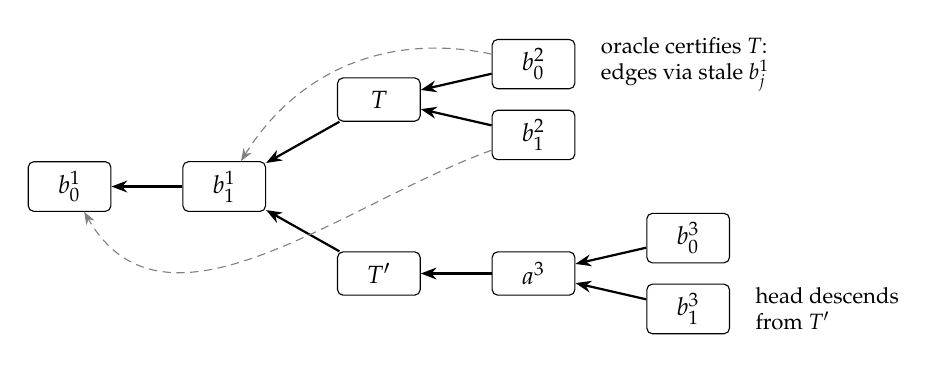
\begin{tikzpicture}[
  blk/.style={draw,rounded corners=2pt,minimum width=1.05cm,minimum height=0.55cm,font=\small},
  par/.style={-{Stealth[length=2mm]},thick},
  jus/.style={-{Stealth[length=1.6mm]},densely dashed,gray},
  node distance=0.55cm and 0.9cm]
\node[blk] (b01) {$b_0^1$};
\node[blk,right=of b01] (b11) {$b_1^1$};
\node[blk,above right=0.5cm and 0.9cm of b11] (T) {$T$};
\node[blk,below right=0.5cm and 0.9cm of b11] (Tp) {$T'$};
\node[blk,right=of T,yshift=0.45cm] (b02) {$b_0^2$};
\node[blk,right=of T,yshift=-0.45cm] (b12) {$b_1^2$};
\node[blk,right=of Tp] (a3) {$a^3$};
\node[blk,right=of a3,yshift=0.45cm] (b03) {$b_0^3$};
\node[blk,right=of a3,yshift=-0.45cm] (b13) {$b_1^3$};
\draw[par] (b11) -- (b01);
\draw[par] (T) -- (b11);
\draw[par] (Tp) -- (b11);
\draw[par] (b02) -- (T);
\draw[par] (b12) -- (T);
\draw[par] (a3) -- (Tp);
\draw[par] (b03) -- (a3);
\draw[par] (b13) -- (a3);
\draw[jus] (b02) to[bend right=35] (b11);
\draw[jus] (b12) to[out=200,in=-60] (b01);
\node[font=\footnotesize,align=left,anchor=west] at ([xshift=0.2cm]b02.east)
  {oracle certifies $T$:\\ edges via stale $b_j^1$};
\node[font=\footnotesize,align=left,anchor=west] at ([xshift=0.2cm]b13.east)
  {head descends\\ from $T'$};
\end{tikzpicture}
\caption{The schedule for $k=2$. Solid arrows are main parents; dashed arrows
are the stale views $\mathit{lm}_{b_i\to b_j}=b_j^1$ that the oracle accepts as
edges.}
\label{fig:counter}
\end{figure}

A re-implementation of the node's edge rule and of LMD-GHOST, independent of
the node and included with this note as \texttt{oracle\_sim.py}, reproduces
the schedule. With $k=10$ it certifies $T$ at $\mathrm{FT}\approx0.832$, above
the default threshold $0.67$ (\texttt{defaults.conf}, with the synchrony
constraint threshold at its default of $0$), and then certifies the sibling
$T'$ at $\mathrm{FT}=1$. With $k=3$ the figures are $0.597$ and $1$. Under the
rule $(\dagger)$ the first certificate has no edges, and the oracle's figure for
$T$ is negative. Equivocating weight is zero throughout, so this violates
Corollary~\ref{cor:finality}, not only its accountable form: two honest
observers finalize incompatible blocks and there is nobody to slash.

\begin{remark}[Scope of the claim]
The schedule is checked against a re-implementation, not against the node.
It rests on three readings of \texttt{safety/clique\_oracle.rs}:
\begin{itemize}[leftmargin=1.5em]
\item no test of $\mathit{lm}_{a\to b}$ against the target when edges are
  computed;
\item the stopper rule and the two-sided height test in the disagreement walk;
\item agreement as main-spine membership.
\end{itemize} A regression test in the node's
finalized-floor suite that builds this DAG is the next step. The Rocq
development is consistent with the finding: its capstones are disclosed as
proving determinism of the floor, not CBC finalization safety, and its
accountable-safety theorem takes the incompatibility hypothesis as an
assumption over a single snapshot.
\end{remark}

\subsection{Repair}

Require $(\dagger)$: in each direction, also check that $\mathit{lm}_{a\to b}$
has the target on its main-parent spine, and treat every visited block that
does not as disagreeing, whatever its height. In code, the walk must include
its lower endpoint, and the below-height branch must return disagreement for
blocks on the target's own spine.

This undoes the relaxation that was introduced to cure a finality stall, in
which a stale window in one validator's view held certification back. Under
Theorem~\ref{thm:clique} that stall was the oracle being right: a validator
whose view of $b$ predates $T$ is not yet held by $b$'s weight, and
certification must wait until its view is refreshed. A positive synchrony
constraint threshold forces such refreshes and shortens the wait; it does not
replace the check, since it is a configuration choice and its default is $0$.

% =====================================================================
\section{What the group contributes}\label{sec:group}

The group action earns its place in three ways, and it is worth being plain
about where it does not.
\begin{itemize}[leftmargin=1.5em]
\item \emph{Signer as datum.} The name of a block records who signed it, and
  the frame of its structure agrees with the datum. Reading a block from any
  validator is one decoder bank, invariant under rotation.
\item \emph{One program.} The honest network is an orbit product of a single
  program, and the protocol's symmetry under relabelling of validators is a
  theorem of the calculus (Proposition~\ref{prop:equiv}), with the
  symmetry-reduction quotient of~\cite[\S5]{oriented} available to a model
  checker. It also locates the one place where symmetry must be broken.
\item \emph{Signatures as frames.} Unforgeability becomes a syntactic
  discipline: a validator speaks only in its own frame.
\end{itemize}
The cancellation behaviour of the oriented communication rule plays no part:
by Lemma~\ref{lem:faithful} every communication with an honest receiver is
between equal names. Neither do chaos and summation. A model in the plain rho
calculus with a signer field on names would prove the same safety theorems.
What it would lose is the statement that the validators are one program.

% =====================================================================
\section{Further work}\label{sec:further}

\begin{itemize}[leftmargin=1.5em]
\item \emph{Mechanisation.} Sections~\ref{sec:blocks}, \ref{sec:safety} and
  \ref{sec:clique} are first-order and finitary, and fit the existing Rocq
  developments. Theorem~\ref{thm:clique} is the theorem the finalized-floor
  dossier lists as out of scope.
\item \emph{Multi-parent merging.} Lemma~\ref{lem:ghost} uses main-parent
  spines and is indifferent to secondary parents. Whether finality of a block
  on the spine gives finality of the effects merged into it is a separate
  question about the merge, which the model does not reach.
\item \emph{Identity-frame presentation.} The decoder bank reads foreign frames
  by enumerating $G$. Frame-fixing with dynamic decorations,
  $\fr{\delta^{-1}}{X}$ in the notation of~\cite[\S6]{oriented}, would read
  every frame with one receive, at the price of the word problem for $G$,
  which is trivial for finite $G$.
\item \emph{Liveness.} Nothing here is about liveness, which in an
  asynchronous setting requires the synchrony assumptions that the model
  deliberately leaves out.
\item \emph{Hash pointers.} Replace quoted closures by names that refer to
  blocks without containing them, with a persistent \emph{seen} fact per block
  and dependency waits as joins. Proposition~\ref{prop:futures} then needs a
  fetch protocol, and Lemma~\ref{lem:dag} needs collision resistance as a
  hypothesis.
\item \emph{Slashing.} Close the loop from $\mathit{ev}$ to the bond map, so
  that the fault weight seen by the estimator falls when evidence is acted on.
\end{itemize}

\section*{Acknowledgements}
This note was drafted in collaboration with Claude (Anthropic).

\begin{thebibliography}{99}
\bibitem{lehmann-rabin}
D.~Lehmann and M.~O. Rabin.
\newblock On the advantages of free choice: a symmetric and fully distributed
  solution to the dining philosophers problem.
\newblock In \emph{POPL}, pages 133--138. ACM, 1981.

\bibitem{oriented}
L.~G. Meredith.
\newblock Oriented processes: group-valued data, a chaos constant, and an
  equivariant COMM for the reflective higher-order calculus.
\newblock F1R3FLY.io research note, draft 3, 2026.

\bibitem{rho}
L.~G. Meredith and M.~Radestock.
\newblock A reflective higher-order calculus.
\newblock \emph{Electronic Notes in Theoretical Computer Science},
  141(5):49--67, 2005.

\bibitem{cbc}
V.~Zamfir, N.~Rush, A.~Asgaonkar, and G.~Piliouras.
\newblock Introducing the ``minimal CBC Casper'' family of consensus protocols.
\newblock Ethereum research, 2018.

\bibitem{tfg}
V.~Zamfir.
\newblock Casper the friendly ghost: a correct-by-construction blockchain
  consensus protocol.
\newblock Ethereum research, 2017.
\end{thebibliography}

\end{document}
